\subsection{Resolved Top Tagging}
\label{subsec:sel_toptag_resolved}

This analysis relies on the identification of resolved top decays. The resolved top decays are defined as consisting of three jets, each separately clustered by the anti-$k_{T}$ algorithm with size parameter R = 0.4. These AK4CHS jets employ charged hadron subtraction to reduce pileup contamination. Each jet is required to have a $\pt$ of at least $30\:\GeV$ and be located within the detector volume.

The resolved top tagging tool used in this analysis is a boosted decision tree (BDT) based multivariate discriminator (MVA), trained using the \textit{Toolkit for Multivariate Data Analysis with ROOT} (TMVA version 4.2.0) \cite{tmva}. The events selected for MVA training are from SM $\ttbar$ processes simulated in the Phys14 MC sample TTJets\_MSDecaysCKM\_central\_Tune4C\_13TeV-madgraph-tauola with a total cross-section of 831.76 pb. We use single lepton $\ttbar$ events and focus on the top where the W boson decays hadronically into two quarks which fragment and hadronize into jets. We permute all combinations of three jets from each event. Each jet from the tri-jet com bination is matched to a generator level parton which is within $\Delta R$ = 0.3 of the jet. 

The training of the MVA exploits the properties of the resolved top decay kinematics and jet identification properties. The jet properties used in the MVA training include a b-tagging discriminant value. This is determined via the most recent version of the \textit{Combined Secondary Vertex} algorithm (v2) together with the \textit{Inclusive Vertex Finder} algorithm (CSVv2+IVF). Although no explicit cut is applied on the b-tag discriminant for the selection of training events, we denote the jet with the highest CSVv2+IVF value as the b jet candidate. The remaining two jets are denoted as candidates for the jets emitted by the hadronic decay of the W boson. Other variables used in the training include the \textit{Quark-Gluon Likelihood} value of each jet, a value that corresponds to whether a jet originated from a quark or a gluon. The opening angles between the resolved top decay jets are also used. These include the separation in $R$- and $\phi$-space between each W decay jet candidate and the b jet candidate. 

We also employ a kinematic fit to the selected combination of three jets, and from this extract a fit probability \cite{kinfit}. We consider the invariant mass of the system comprised of the two candidate jets for the hadronic decay of the W boson. We also consider the three-jet system which includes the b jet candidate. The invariant masses of the two- and three-jet systems are constructed and the four-vectors of the jets are allowed to vary within their respective uncertainties in order to satisfy the top quark and W boson mass constraints imposed. A minimized $\chi^{2}$ function is extracted from the convergence of the kinematic fit and translated into a probability of fit. 

The input variables used in the training of the resolved top tagger include:
\begin{itemize}
\item jet CSVv2+IVF
\item jet quark-gluon likelihood (QGL)
\item $\Delta R$ ( hadronic W decay jet$_{\mbox{\scriptsize{1,2}}}$, b jet )
\item $\Delta \phi$ ( hadronic W decay jet$_{\mbox{\scriptsize{1,2}}}$, b jet )
\item fit probability 
\end{itemize}

and the jets selected for training satisfy the following requirements: 
\begin{itemize}
\item 3 AK4CHS jets with $\pt>30\:\GeV$ and $|\eta|<2.4$	
\item $100\:\GeV<M_{\mbox{\scriptsize{jjj}}}<300\: \GeV$
\end{itemize}

The MVA is trained with 100,000 signal events and 200,000 background events using the decision tree method which implements the \textit{GradientBoost} algorithm. A \textit{shrinkage} parameter, the learning rate for the GradientBoost algorithm, of 0.05 is specified. The small shrinkage necessitates the growth of more decision trees, but can significantly improve the accuracy of a prediction in difficult settings.

Input training variable correlations are shown in Fig.~\ref{fig:corr}. As expected, the kinematic angles $\Delta R$ and $\Delta\phi$ between the W decay candidate jets and the b jet candidate are correlated strongly in the signal, and less so in the background. 

\begin{figure}[htbp]
	\centering
	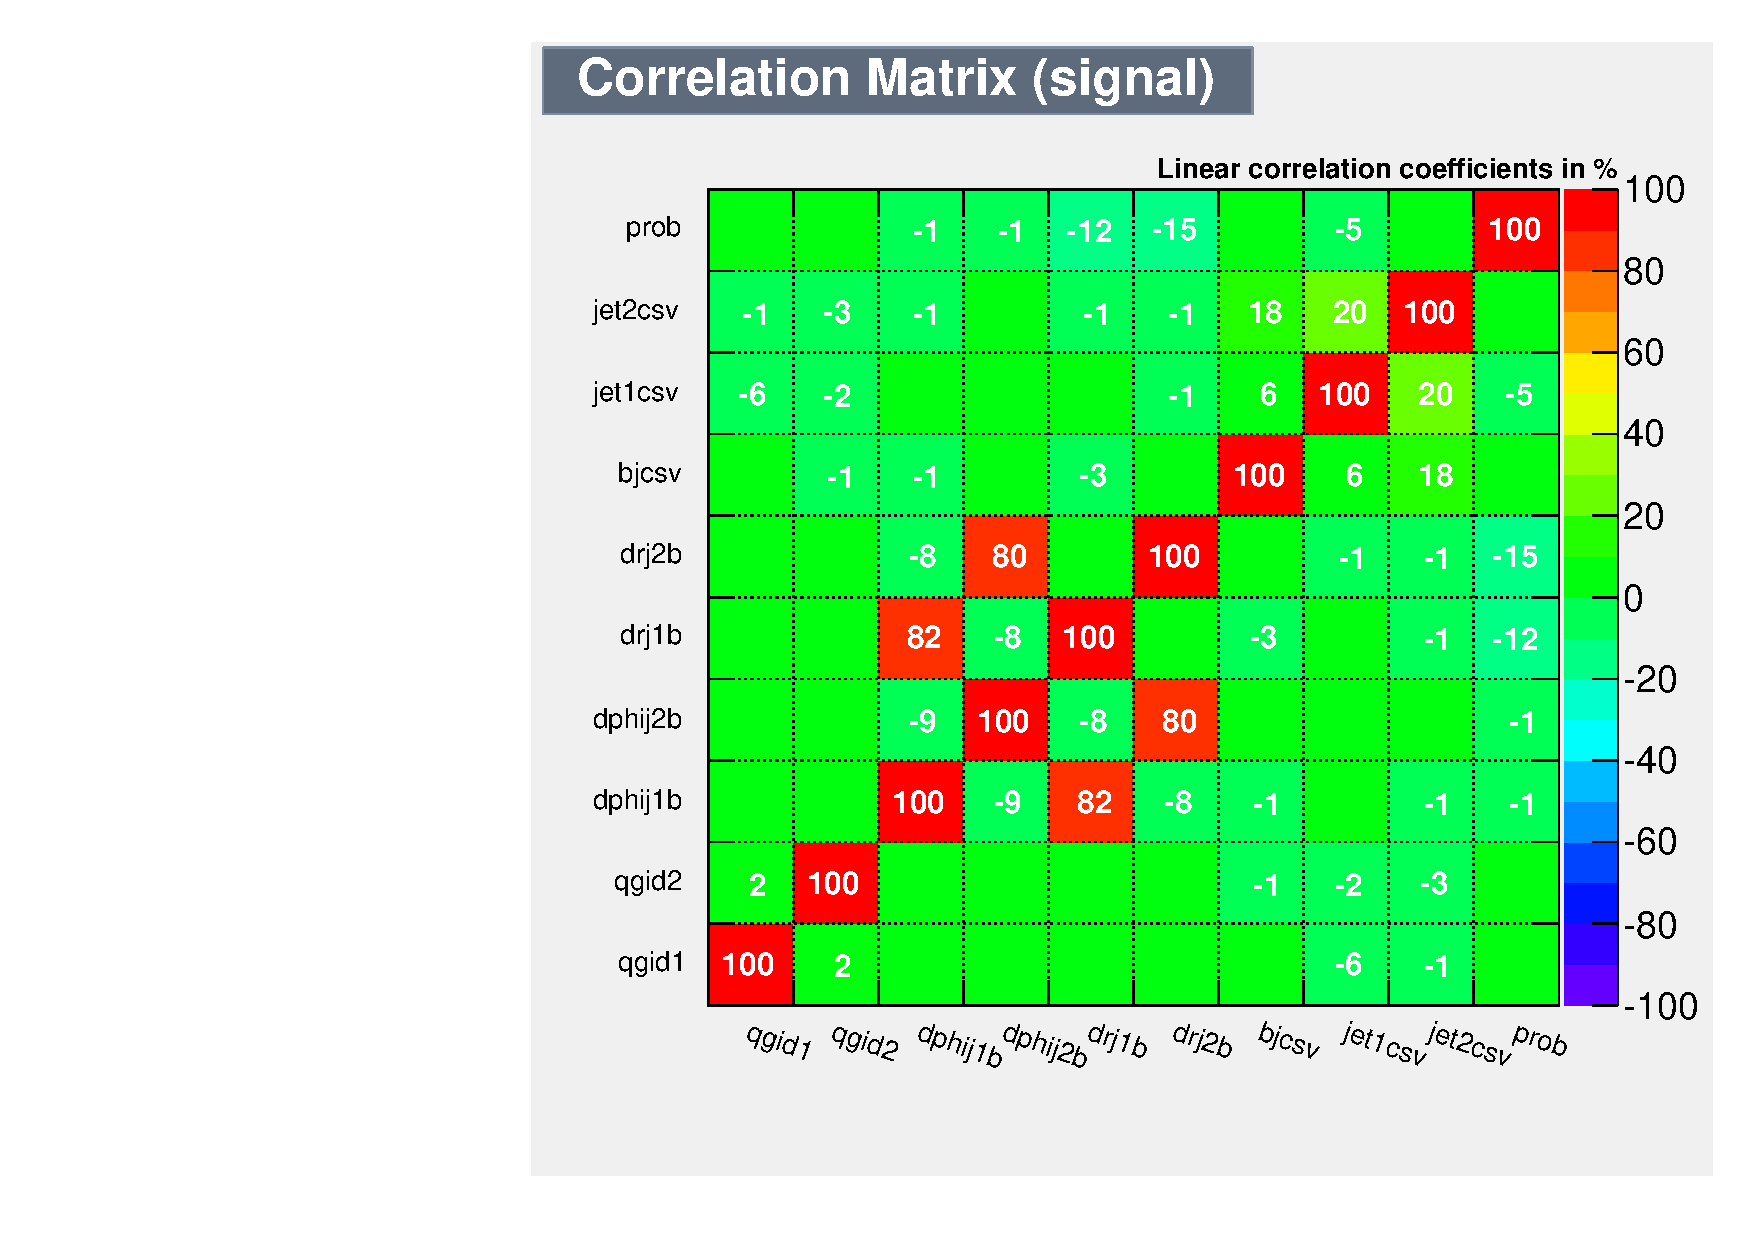
\includegraphics[width=0.48\textwidth]{figures/CorrelationMatrixS.pdf}
	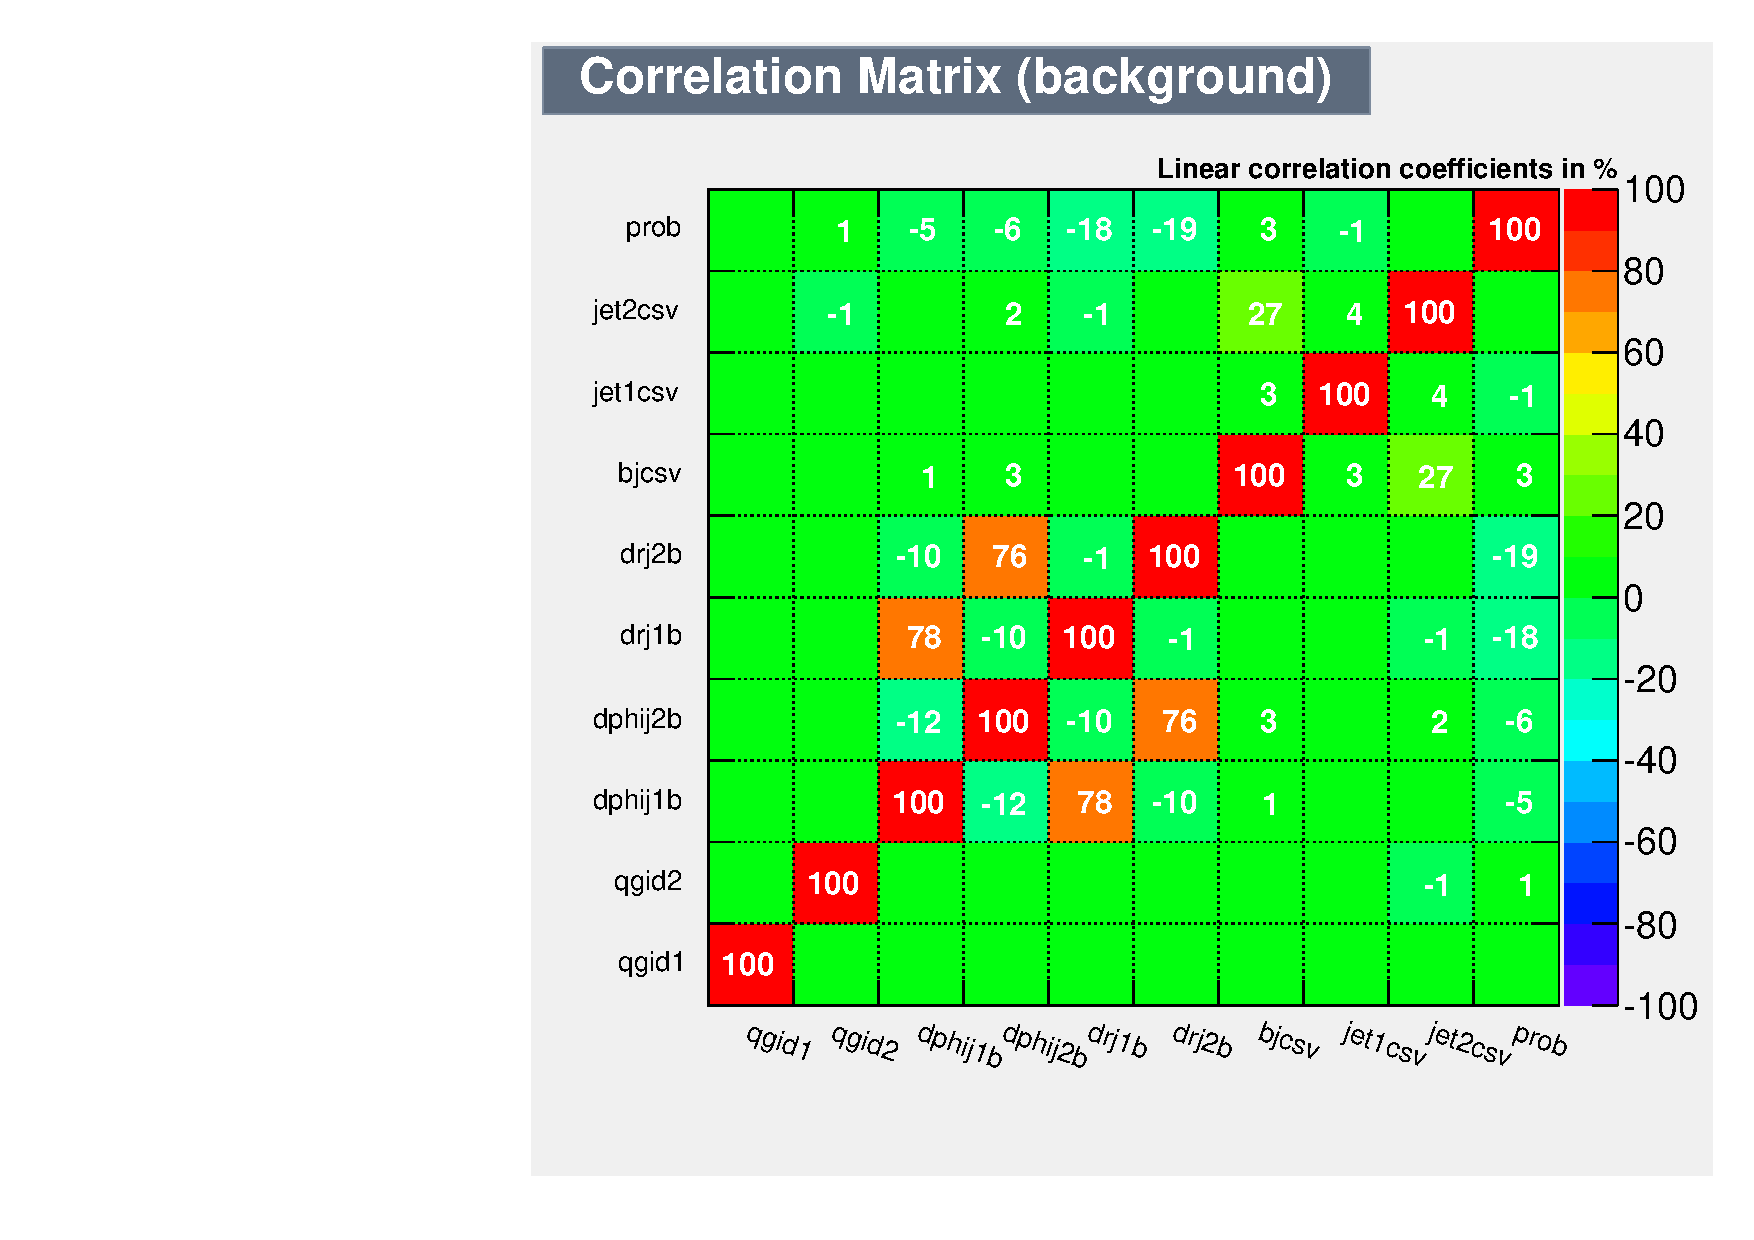
\includegraphics[width=0.48\textwidth]{figures/CorrelationMatrixB.pdf}
	\caption{Correlations between MVA input variables for signal and background}
	\label{fig:corr}
\end{figure}

The performance of the resolved top tagger is evaluated in single lepton $\ttbar$ events and $\Z\To\Nu\Nu$(+jets) events. Unique subsets of the same SM $\ttbar$ MC sample are used to train and test the MVA. A single event can contribute multiple background combinations, thus the tagger is evaluated using the background combination which has the highest output MVA score.

\begin{figure}[htbp]
	\centering
	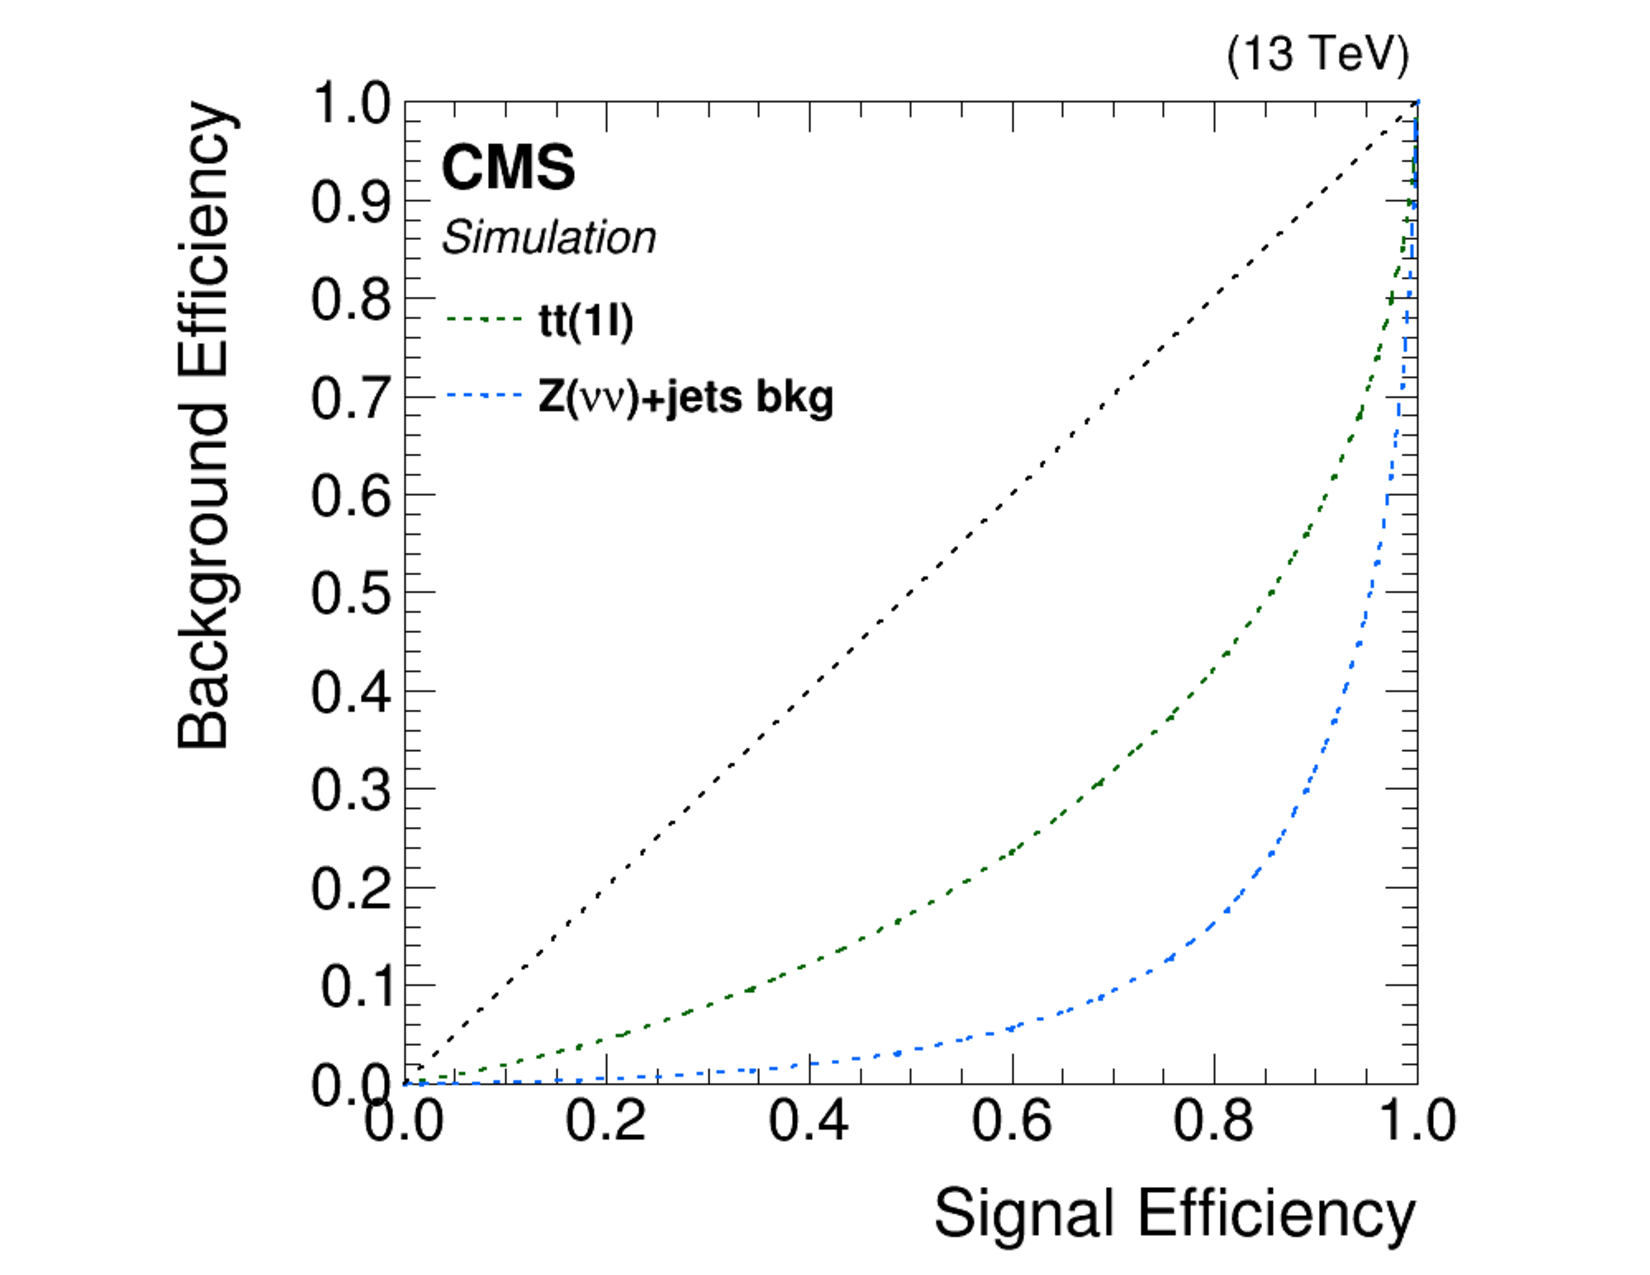
\includegraphics[width=0.48\textwidth]{figures/roctt1lzjets.pdf}
	\caption{Background  vs. signal efficiencies for $\ttbar(1\Lep)$ and $\Z\To\Nu\Nu$(+jets)}
	\label{fig:rocres}
\end{figure}

The efficiency behaviour of the resolved top tagger with respect to increasing top quark \pt\:\ was studied in MC. The efficiency in $\ttbar(1\Lep)$ events, the mistag rate of the $\ttbar(1\Lep)$ combinatoric background, and the mistag rate of $\Z\To\Nu\Nu$ events are shown as a function of the generator level top quark \pt\:\ in Fig.~\ref{fig:eff}. A working point corresponding to an approximate signal efficiency of 60$\%$ in $\ttbar(1\Lep)$ events was chosen as an illustrative benchmark. Limited statistics are available in the high top \pt\:\ regime.

\begin{figure}
	\centering
	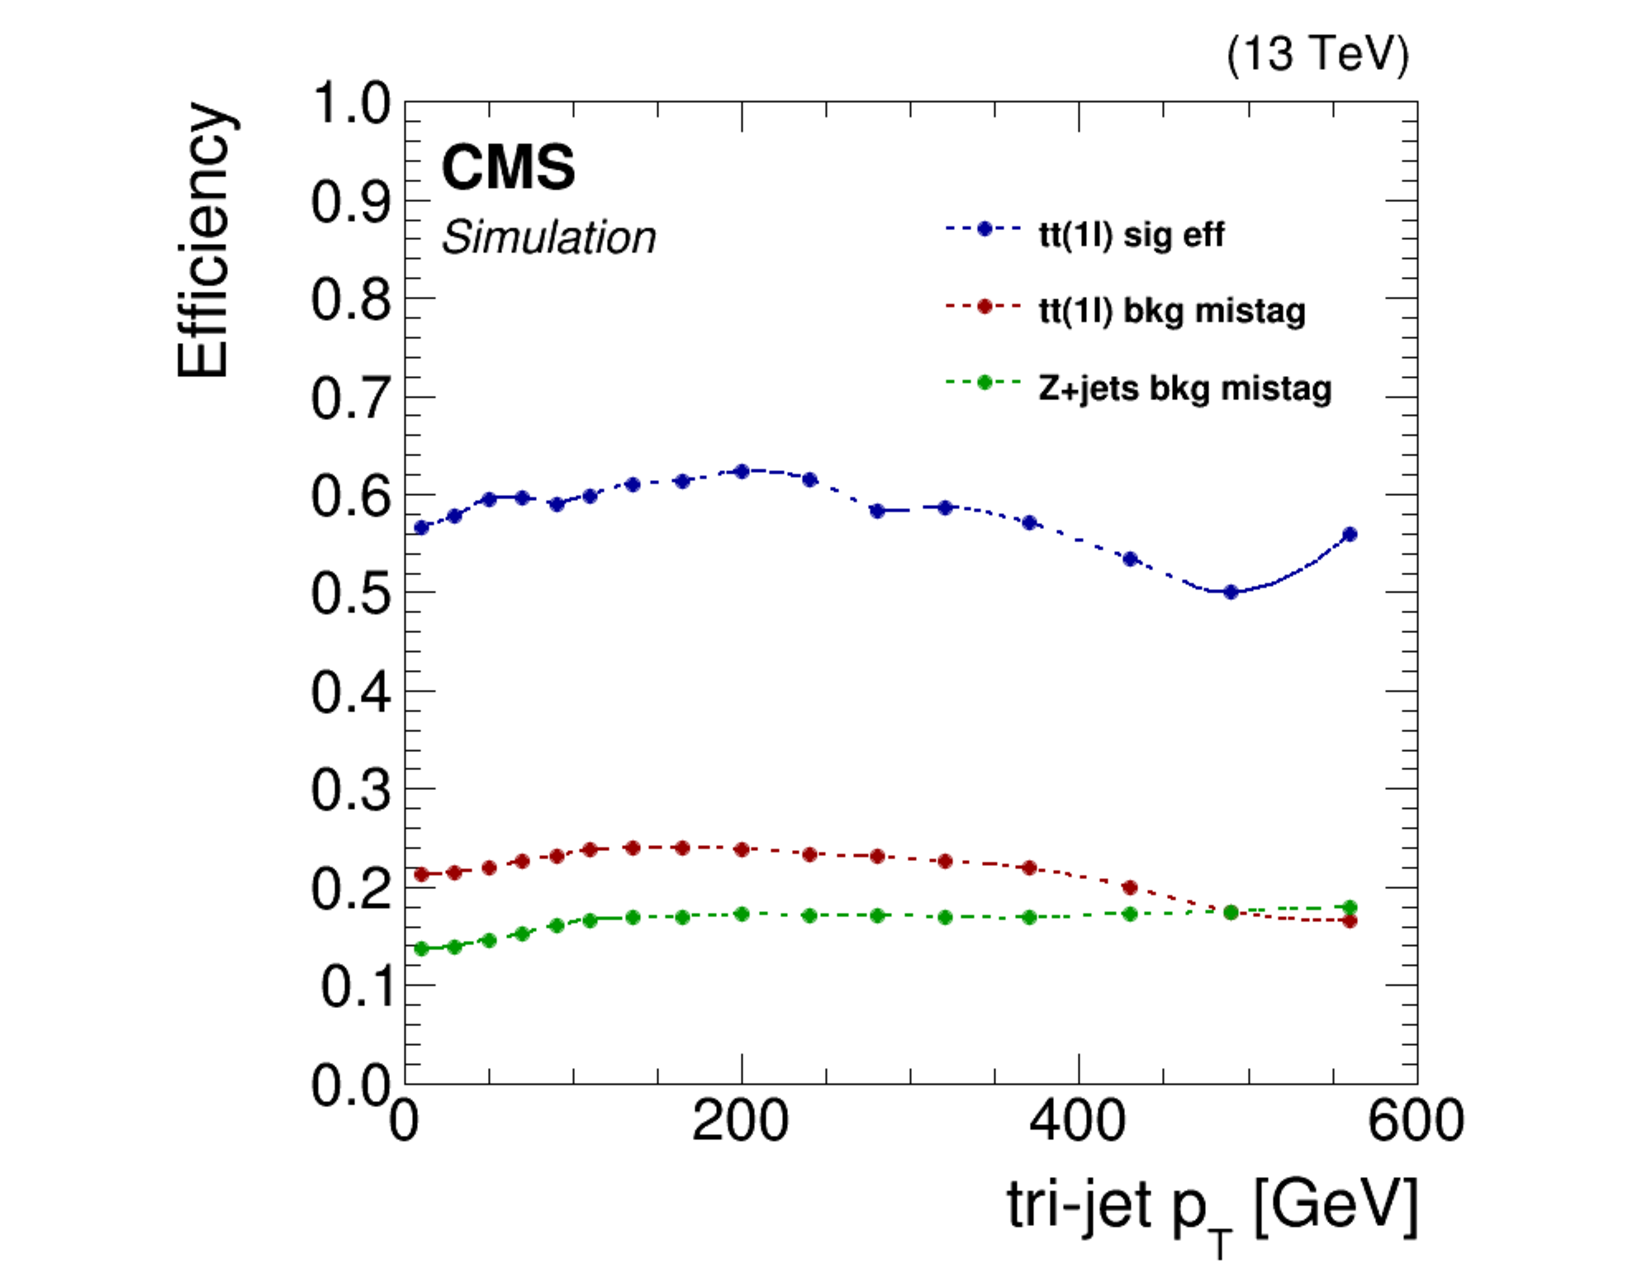
\includegraphics[width=0.48\textwidth]{figures/baseMVA+prob_bkg_effvspt.pdf}
	\caption{Resolved top tagger efficiency and mistag rates in $\ttbar(1\Lep)$ and $\Z\To\Nu\Nu$(+jets) Phys14 MC samples as a function of generator level top quark \pt\:\ and tri-jet \pt\:\ respectively}
	\label{fig:eff}
\end{figure}

The performance of the resolved top tagger was also characterized in 13\:\TeV\: data. Events for the study were selected using the HLT\_IsoMu27 trigger. The events satisfy the following offline selection criteria:

\begin{itemize}
\item exactly one muon passing ``Tight" selection with $\pt>30\:\GeV$ and $|\eta|<2.4$ 
\item $\met>100\: \GeV$
\item $M_T>40\: \GeV$
\item at least three AK4CHS jets with $\pt>30\:\GeV$ and $|\eta|<2.4$ 
\item at least two jets passing the``Medium" CSVv2+IVF WP 
\end{itemize}

The MVA output score distribution for data and MC is shown in Fig.~\ref{fig:score}. 

\begin{figure}[htbp]
	\centering
	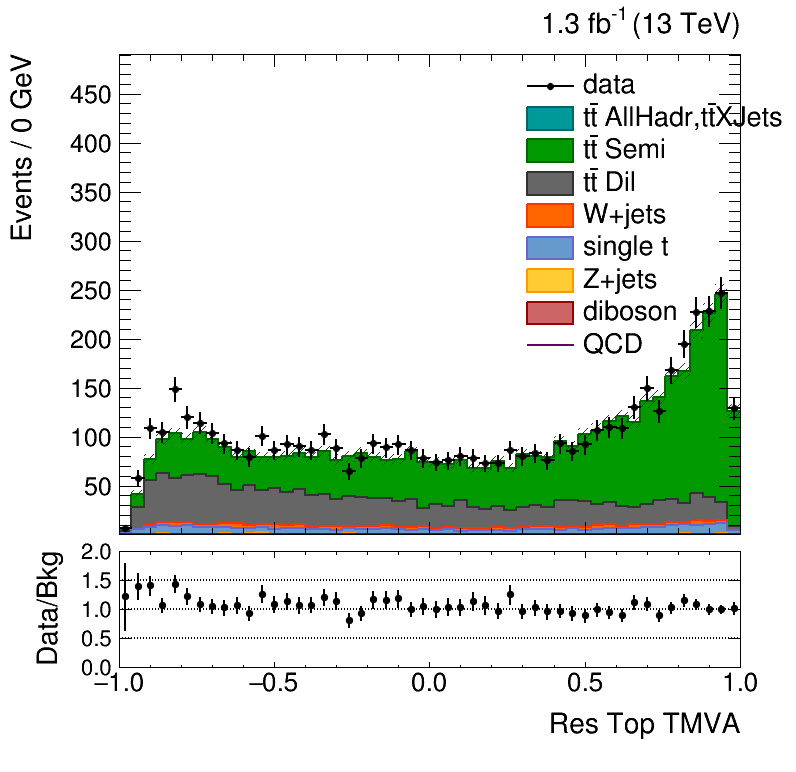
\includegraphics[width=0.48\textwidth]{figures/semilep_1tightmuo_resolved_3ormorejets_2ormorejetWPm_pfmetmore100_pfmtmore40_trigrequestonMC_qgsmearedwith8TeVrecipe_Oct302015/hResTopMVAlinear.png}
	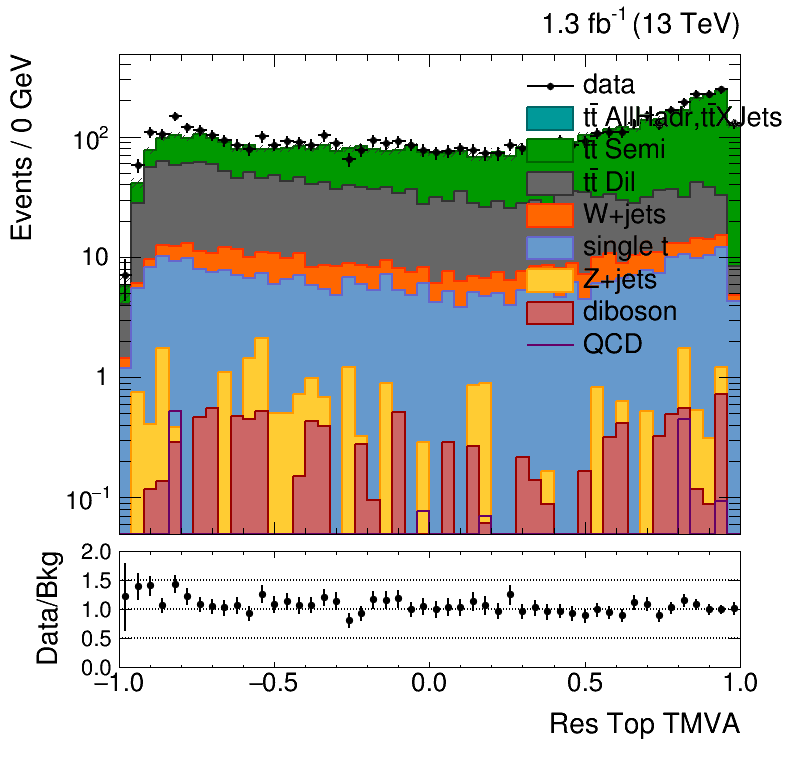
\includegraphics[width=0.48\textwidth]{figures/semilep_1tightmuo_resolved_3ormorejets_2ormorejetWPm_pfmetmore100_pfmtmore40_trigrequestonMC_qgsmearedwith8TeVrecipe_Oct302015/hResTopMVA.png}
	\caption{Resolved top tagger MVA output score distributions in data and MC in linear and log scale}
	\label{fig:score}
\end{figure}

Fair agreement is observed between data and MC, however better agreement is observed in 8\:\TeV\: studies, as described in Appendix ~\ref{app:8TeV}. The likely cause for the discrepancy at low MVA scores is due to the QGL which is currently under inverstigation (see Appendix ~\ref{app:TopTagger13TeVMore}).

In order to measure the efficiency and fake rates in data \footnote{Different efficiency/fake rate definitions used for training/characterization purposes (MC only) and scale factor measurements (data and MC comparison)}, the standard \textit{Tag and Probe} technique is employed \cite{TnP}. The semi-leptonic top candidate in the $\ttbar(1\Lep)$ event is taken to be the ``tag", while the ``probe" is the hadronically decaying top.
 The ``probe" is required to pass the aforementioned jet triplet selection. A passing ``probe" also passes the specified MVA score threshold, whereas a failing ``probe" will have an MVA output score lower than the specified threshold. The efficiency of the resolved top tagger is taken to be the number of passing ``probes" out of the total number of passing and failing ``probes".

In order to determine the yields in these categories, a simultaneous fit is performed in the orthogonal passing and failing ``probe" samples using the \textit{RooFit} framework. A $\ttbar(1\Lep)$ event can contribute either a jet triplet combination wherein each jet is matched to a generator level parton emitted from the hadronic top decay (signal) or a jet triplet combination with jets matched to underlying partons/combinatorial parton mismatch (background). Three  MC mass templates for the passing and failing ``probe" samples are constructed from:

\begin{itemize}
\item $\ttbar(1\Lep)$ signal events
\item $\ttbar(1\Lep)$ combinatorial background events
\item non-$\ttbar(1\Lep)$ background events (W/Z+jets, dibosons, single top, $\ttbar(2\Lep)$, hadronic \ttbar, \ttbar X(jets) )
\end{itemize}		 
	
The fit features six uncostrained nuisance parameters: 
\begin{itemize}
 \item signal rate in the inclusive (pass+fail) sample,
 \item combinatorial-background rate in the inclusive sample,  
 \item non-$\ttbar(1\Lep)$ background rate,
 \item signal efficiency ($\epsilon$), 
 \item combinatorial background fake rate ($FR1$) ,
 \item non-$\ttbar(1\Lep)$ background fake rate ($FR2$). 
 \end{itemize} 
 $\epsilon$, $FR1$, $FR2$ are defined respectively as the relative rates of passing ``probes" in signal, combinatorial-background, and non-$\ttbar(1\Lep)$ background.
 
 Results of the fit versus the chosen MVA score threshold is shown in Fig. \ref{fig:roofitresults13TeV}. Overall, we see good agreement, as in the 8 TeV data in appendix \ref{app:8TeV}.\\ 
  \textcolor{red}{Work on estimating the systematic uncertainties impacting the measurement.}
 
 \begin{figure}[htbp]
	\centering
	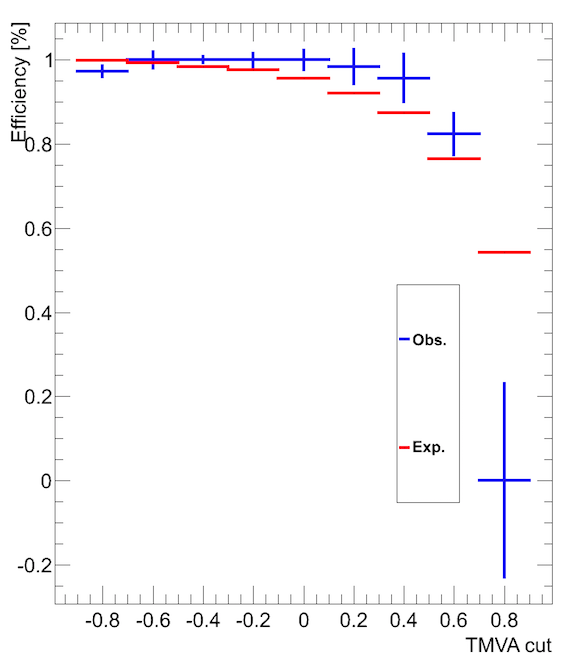
\includegraphics[width=0.48\textwidth]{figures/TOPRESOLVEDTAGGER_13TeV/c_eff.png}\\
	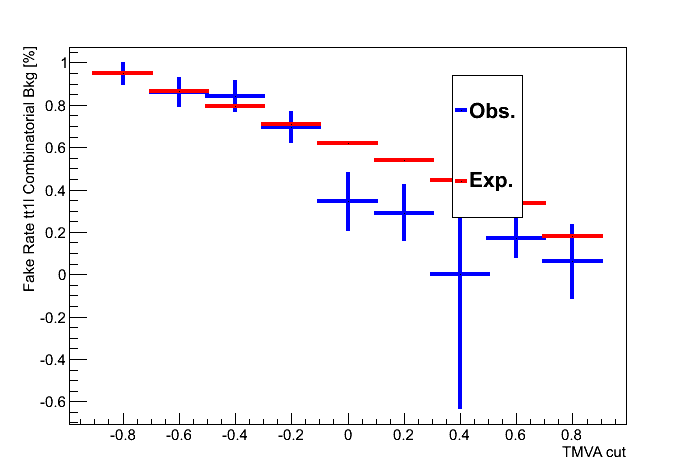
\includegraphics[width=0.48\textwidth]{figures/TOPRESOLVEDTAGGER_13TeV/c_fr1.png}
	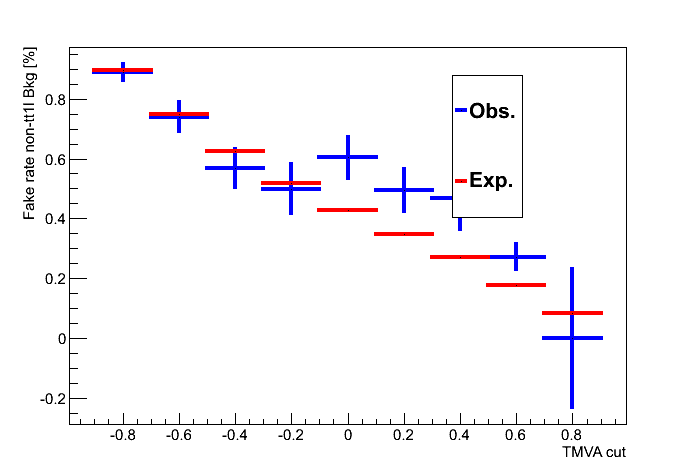
\includegraphics[width=0.48\textwidth]{figures/TOPRESOLVEDTAGGER_13TeV/c_fr2.png}
	\caption{Signal efficiency (top),  combinatorial background fake rate (bottom left), and non-$\ttbar(1\Lep)$ background fake rate (bottom right) in data (blue) and MC (red) as function of the MVA threshold. The procedure to estimate those quantities has been described in the text.}
	\label{fig:roofitresults13TeV}
\end{figure}


















